
%(BEGIN_QUESTION)
% Copyright 2009, Tony R. Kuphaldt, released under the Creative Commons Attribution License (v 1.0)
% This means you may do almost anything with this work of mine, so long as you give me proper credit

Suppose a mechanic pulls perpendicularly at the end of a wrench 0.6 meters in length with a steady force of 190 newtons for two complete revolutions.  Calculate the amount of work done by the mechanic (in newton-meters or joules), and also calculate his power output in watts if those two turns were completed in 6 seconds.

$$\includegraphics[width=15.5cm]{i03777x01.eps}$$

\underbar{file i03777}
%(END_QUESTION)





%(BEGIN_ANSWER)

The mechanic's work is 1432 Newton-meters, or 1432 Joules.  The mechanic's average power output during the 6 seconds is 238.7 watts.

%(END_ANSWER)





%(BEGIN_NOTES)

Rotational work is calculated by the following formula:

$$W = \tau \theta$$

$$W = (190 \hbox{ N})(0.6 \hbox{ m})(4 \pi)$$

$$W = 1432 \hbox{ N-m}$$

\vskip 10pt

Since power is the rate of work done over time, and the time to do this work was 6 seconds, the average power is:

$$\overline{P} = {\Delta W \over \Delta t}$$

$$\overline{P} = {1432 \hbox{ N-m} \over 6 \hbox{ s}}$$

$$\overline{P} = 238.7 \hbox{ W}$$

%INDEX% Physics, energy, work, power: calculating work and power

%(END_NOTES)


